\documentclass[a4paper, 10pt, twoside, openright, openany]{book}
\usepackage[english,italian]{babel}
\usepackage[T1]{fontenc}
\usepackage[utf8]{inputenc}
\usepackage{fancyhdr}
\usepackage{float}
\usepackage{graphicx}
\usepackage{wrapfig}
\usepackage{siunitx} %per scrivere il simbolo °
\usepackage{verbatim} %per i commenti1
\usepackage{subfig}
\usepackage{amsmath}
\usepackage{algorithm}
\usepackage{algpseudocode}
\setcounter{secnumdepth}{3}
\setcounter{tocdepth}{6}
\usepackage{multirow}
\newcommand{\minitab}[2][l]{\begin{tabular}#1 #2\end{tabular}}
\usepackage{rotating}
\usepackage{xfrac}

\DeclareMathOperator*{\argmax}{arg\,max}
\DeclareMathOperator*{\argmin}{arg\,min}

%\usepackage{booktabs,array}
%\usepackage{tikz}

%\usepackage{tabularx}

%\usepackage{chngcntr}
%\counterwithin{table}{section}

%------------------------------ colors
\usepackage[usenames,dvipsnames,table]{xcolor} % use colors on table and more
\definecolor{333}{RGB}{51, 51, 51} % define custom color
\definecolor{background}{RGB}{255, 254, 213}
\definecolor{comment}{RGB}{17,167,5}
\definecolor{keyword}{RGB}{195,47,8}
\definecolor{string}{RGB}{142,195,0}
\definecolor{number}{RGB}{90,84,84}
\definecolor{identifier}{RGB}{0,90,201}

%------------------------------ source code
\usepackage{listings}

\lstset{
  basicstyle=\footnotesize\sffamily,
  commentstyle=\itshape\color{gray},
  captionpos=b,
  frame=shadowbox,
  language=HTML,
  rulesepcolor=\color{333},
  tabsize=2
}

\lstdefinestyle{code}{
  backgroundcolor=\color{background},
  basicstyle=\footnotesize\sffamily,
  commentstyle=\color{comment},
  frame=L,
  identifierstyle=\color{identifier},
  keywordstyle=\color{keyword},
  numbers=left,
  numbersep=10pt,
  numberstyle=\tiny\color{number},
  stringstyle=\color{string},
  showstringspaces=false,  
  stepnumber=1,
  tabsize=2
}


%------------------------------ define Abstract environment, missing in the 'book' class
\newenvironment{abstract}{\cleardoublepage \null \vfill \begin{center}\bfseries\abstractname \end{center}}{\vfill\null}
\addto\captionsenglish{\renewcommand*\abstractname{Abstract}} % change Abstract title

%------------------------------ active url
\usepackage{url}
\renewcommand{\UrlFont}{\color{black}\small\ttfamily}
\usepackage[colorlinks=true, linkcolor=black, citecolor=black, urlcolor=black]{hyperref} % active ref
%------------------------------ macros
\newcommand{\sectionname}{Section} % define Section ref
\newcommand{\subsectionname}{Sub-section} % define Sub-section ref
\renewcommand*\arraystretch{1.4} % tables padding

%acronimi
\usepackage[printonlyused]{acronym}

\begin{document}
\frontmatter

\begin{titlepage} %------------------------------ TITLE PAGE
\begin{center}


\hspace{0.5cm}
\begin{minipage}{.20\textwidth}
  
\includegraphics[height=2.5cm]{./Images/Utility/UNIPD}
\end{minipage}\begin{minipage}{.90\textwidth}
  \begin{table}[H]
  \begin{tabular}{l}
  \scshape{\Large{\bfseries{Università degli Studi di Padova}}} \\
  \hline \\
  \scshape{\Large{Facoltà di Ingegneria}} \\
  \end{tabular}
  \end{table}
\end{minipage}

\vspace{1cm}
\emph{\Large{Corso~di~Laurea~Magistrale~in~Ingegneria~Informatica}} \\
\vspace{3cm}
\scshape{\Large{Relazione di CALCOLO PARALLELO}} \\
\end{center}

\vspace{1cm}
\begin{center}
\scshape{\Large{\bfseries{BitonicSort VS QuickSort}}}
\end{center}

\vspace{3.5cm}

\begin{center}
\emph{Autori}
\vspace{0.2cm}
\begin{table}[h]
\centering
\begin{tabular}{rl}
\vspace{0.2cm}
{Matteo Perin} & {******}\\
{Davide Pistilli} & {1204880}\\
{Flavio Spanò} & {1197697}\\
\end{tabular}
\end{table}

\end{center}

\vfill
\begin{center}
\hspace{-0.2cm}
\line(1, 0){360}\\
\textsc{Anno Accademico 2018-2019}
\end{center}
\end{titlepage}

\begingroup %------------------------------ CONTENTS
  \makeatletter
  \let\ps@plain\ps@empty
  \makeatother
  \tableofcontents  
  \clearpage
\endgroup

\mainmatter
\chapter{Introduzione}

L'ordinamento è uno dei problemi cardine di innumerevoli applicazioni scientifiche e ingegneristiche e le prestazioni degli algoritmi che lo risolvono sono di diretto interesse pratico.

Molti algoritmi sequenziali richiedono un tempo $O(NlogN)$ per eseguire l'ordinamento. Per aumentare la velocità di queste operazioni sono stati ideati alcuni metodi paralleli che sfruttano la presenza di più processori che possono svolgere operazioni in contemporanea e comunicare tra di loro.

In questa relazione verranno analizzate e messe a confronto le prestazioni di due algoritmi parallelizzati: il \textit{Bitonic Sort} e il \textit{Quick Sort}. Le due implementazioni includono le ottimizzazioni proposte, rispettivamente, in \cite{PaperBitonic} e \cite{PaperQuickSort}.

\chapter{DescrizioneAlgoritmo}


\begin{document}



\maketitle QuickSort

Quicksort è un algoritmo di ordinamento sequenziale ampiamente ritenuto essere l'algoritmo di ordinamento sequenziale più veloce per un ampio set di input, infatti il termine che tradotto letteralmente in italiano indica ordinamento rapido. È l'algoritmo di ordinamento che ha, nel caso medio, prestazioni migliori tra quelli basati su confronto. È stato ideato da Charles Antony Richard Hoare nel 1961.\\ 
È un algoritmo ricorsivo che usa il metodo "Divide and Conquer" per ordinare tutti i valori. Quicksort dal momento che scompone ricorsivamente i dati da processare in sottoprocessi, tale procedura viene chiamata Partition, preleva prima un pivot da una struttura dati, trova la sua posizione nell'elenco in cui deve essere posizionata. \\
Avremo due possibilità:
\begin{itemize}
\item I valori minori del pivot saranno posizionati nella parte sinistra dell'array
\item I valori maggiori o uguali saranno posizionati nella parte di destra dell'array
\end{itemize}




\maketitle Bitonic Sort



\end{document}
\chapter{Bitonic Sort} \label{chap.BitonicSort}

\section{Funzionamento generale}

L'algoritmo di \textit{Bitonic Sorting} produce una sequenza ordinata dopo alcune iterazioni di \textit{Bitonic Merge}, che convertono due sequenze bitoniche di grandezza \textit{m} in un'unica sequenza monotona di grandezza \textit{2m}.
La figura \ref{bitonic1} mostra una rete di ordinamento bitonico per 8 valori.

\begin{figure}[h!]
  \centering
  \includegraphics[width=\linewidth]{Images/bitonic1.png}
  \caption{Rete di ordinamento bitonico per 8 valori}
  \label{bitonic1}
\end{figure}

Ogni segmento verticale rappresenta un comparatore a 2 ingressi e 2 uscite e con una sua polarità, il quale svolge un'operazione \textit{Compare and Exchange}. Un comparatore con la freccia verso il basso restituisce il valore più alto alla porta più bassa e viceversa. Un comparatore con la freccia verso l'alto, invece, restituisce il valore più alto alla porta più bassa e viceversa.

\section{Implementazione parallela}

Nella mappatura del \textit{Bitonic Sort} su architetture parallele ogni comparatore è sostituito da una coppia di processori che svolgono un'operazione chiamata \textit{Merge and Split}. Ogni processore è a carico di un numero $n = N / P$ di valori, di cui ne mantiene una lista ordinata durante l'esecuzione. La figura \ref{bitonic2}, ad esempio, mostra l'ordinamento di 16 valori con 4 processori.

\begin{figure}[h!]
  \centering
  
\includegraphics[width=\linewidth]{Images/bitonic2.png}
  \caption{Esempio di rete bitonica su archiettura parallela}
  \label{bitonic2}
\end{figure}

In un'operazione di \textit{Merge and Split}, date in ingresso due sequenze ordinate, esse vengono unite in un'unica sequenza ordinata, che sarà poi sezionata nella sua parte maggiore e parte minore. Ogni processore terrà in memoria solo la parte maggiore (polarità \textit{U}) o minore (polarità \textit{L}) in base alla sua polarità (direzione della freccia), similmente a quanto accadeva nell'operazione \textit{Compare and Exchange}.

L'algoritmo fa in modo che ogni processore mantenga lo stesso numero di dati, quindi bilancia perfettamente il carico di lavoro in ogni ciclo. D'altra parte, se è implementato in un sistema parallelo a memoria distribuita, una grande porzione del tempo è dedicata alle comunicazioni interprocessore. Questo è causato dal fatto che l'algoritmo richiede che ogni processore scambi tutti i suoi dati durante la fase \textit{Merge and Split}.

Per questo in \cite{PaperBitonic} si è cercato di ridurre il numero di dati da scambiare in tali fasi. Invece di inviare tutti i suoi $n$ valori, infatti, ogni processore può inviare solo i dati effettivamente necessari. Dato che, alla fine dell'iterazione, un processore terrà solo una parte del risultato del \textit{merging}, sarà necessario inviare solo le chiavi necessarie a determinare questa lista di $n$ valori. Inizialmente, ogni coppia di processori scambia con l'altro il suo valore minimo se ha polarità U, il suo valore massimo se ha polarità L. Dato che sicuramente il processore con polarità L non terrà i valori che sono maggiori del suo massimo, il processore con polarità U può inviare a quest'ultimo solo i valori minori di tale massimo. Similmente, dato che sicuramente il processore con polarità U non terrà i valori che sono minori del suo minimo, il processore con polarità L può inviare a quest'ultimo solo i valori maggiori di tale minimo. Considerando il valore ricevuto dall'altro processore, vengono quindi inviati solo i valori che effettivamente hanno una possibilità di entrare nella lista alla fine dell'iterazione.

Successivamente, il processore L sceglierà semplicemente i valori più piccoli tra quelli inviati e quelli ricevuti da U e viceversa.

Un esempio dell'intero procedimento può essere visto in figura \ref{mergeAndSplit}.

\begin{figure}[h!]
  \centering
  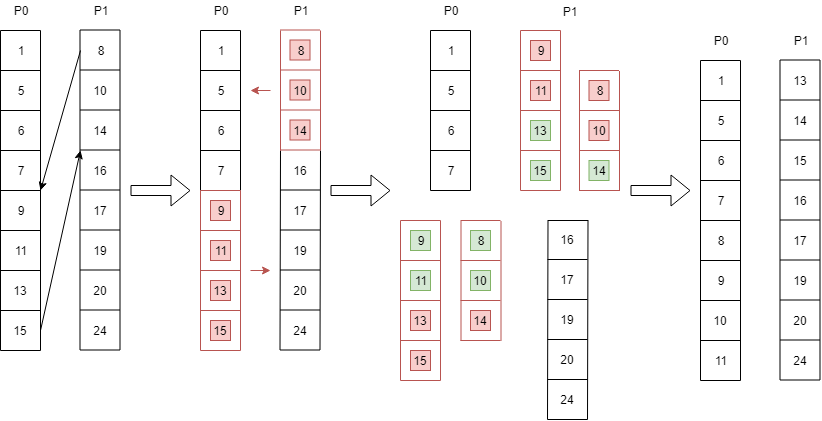
\includegraphics[width=\linewidth]{Images/mergeAndSplit.png}
  \caption{Fase modificata di Merge and Split}
  \label{mergeAndSplit}
\end{figure}

La riduzione del numero di valori da trasferire nel canale di comunicazione si dovrebbe tradurre in un aumento delle prestazioni. La ricerca del valore e la preparazione del buffer da trasferire introducono però operazioni aggiuntive a ogni iterazione. Il vantaggio sussiste, di conseguenza, solo se la taglia del problema rende il risparmio sulla comunicazione maggiore dell'\textit{overhead} introdotto.

\subsection{Descrizione dell'implementazione}

L'implementazione utilizzando \textit{MPI} segue quasi alla lettera il procedimento appena descritto.

Ricevuta la sequenza da ordinare, il processore \textit{MASTER} divide equamente i valori tra tutti i processori.

Dopodiché, ogni processore ordina la lista di valori ricevuta utilizzando l'ordinamento bitonico sequenziale (in \cite{PaperBitonic} venivano invece generate sequenze ordinate direttamente in ogni processore, ma si è deciso di seguire la strada dell'ordinamento per rendere il funzionamento del programma affine a quello del \textit{Quick Sort}, descritto nel prossimo capitolo).

L'implementazione del Bitonic Sort è di tipo iterativo, ottenendo un risparmio in memoria primaria. Per determinare quali sono le coppie su cui si svolge l'operazione di \textit{Compare and Exchange} viene utilizzato il seguente metodo: k seleziona la posizione del bit che determina se la coppia di elementi deve essere scambiata in ordine crescente o decrescente, la variabile j corrisponde alla distanza a cui devono essere gli elementi interessati al \textit{Compare and Exchange}, la variabile i iterata su tutti gli elementi, $i XOR j$ è l'elemento accoppiato a i (cioè l'elemento la cui posizione differisce solo per il bit in posizione $log_2 j$). Viene fatto il confronto solo se $i < ixj$, in modo da non ripetere lo stesso confronto due volte.

Dopo questo passo ogni processore contiene una sequenza ordinata di $n = N / P$ valori, si può quindi procedere con l'algoritmo parallelo descritto precedentemente. 

Per determinare il rango dei processori che devono comunicare viene utilizzato un metodo del tutto simile a quello applicato per l'ordinamento sequenziale. A ogni iterazione i processori accoppiati si mettono in comunicazione e svolgono il processo di \textit{Merge and Split} chiamando la funzione \textit{void mergeAndSplit(int in[], int rank, int r\_min, int r\_max, int num\_keys)}. Il ruolo di ogni processore viene determinando passando il suo rango come parametro in r\_max se ha polarità U o in r\_min altrimenti. Il processore con cui si comunica viene determinando passando il suo rango come parametro in, rispettivamente, r\_min o r\_max.

All'interno di questa funzione ogni processore seguirà una strada diversa in base alla polarità assegnata al suo rango. Le due strade sono simmetriche tra loro e corrispondono a quelle illustrate in figura \ref{mergeAndSplit}.

In base alla polarità ogni processore invia, a questo punto, il suo massimo o minimo al suo compagno. Una volta ricevuto il valore ogni processore esegue una ricerca binaria iterativa per trovare all'interno dei suoi dati il primo valore maggiore o uguale a quello ricevuto, l'indice relativo viene salvato nella variabile $c$.

Vengono quindi preparati i buffer per l'invio dei dati: il processore con polarità L invierà solo i dati da $c$ a $n - 1$, il processore con polarità U quelli da $0$ a $c$.

Una volta ricevuti i dati ogni processore mantiene i valori massimi o minimi presenti nel buffer inviato e in quello ricevuto in base alla sua polarità e li inserisce nel vettore dei suoi valori mantenendone l'ordinamento.

Una volta terminate tutte le iterazioni il processore \textit{MASTER} raccoglie tutti i dati e ottiene quindi la sequenza ordinata che viene restituita al processo chiamante.

\chapter{Quicksort} \label{chap.QuickSort}
\section{Funzionamento generale}
Quicksort è un algoritmo di ordinamento sequenziale ampiamente utilizzato grazie alla sua velocità e semplicità. Il suo nome significa "ordinamento rapido" e, infatti, è l'algoritmo di ordinamento con le prestazioni migliori, nel caso medio, tra quelli basati su confronto.
Si tratta di un algoritmo ricorsivo che sfrutta il paradigma \textit{Divide and Conquer}: prima i dati vengono scomposti ricorsivamente in base ad un valore chiave chiamato \textit{pivot}. I valori minori o uguali al pivot saranno posizionati nella parte sinistra del sottoarray considerato, mentre i valori maggiori o uguali saranno posizionati nella parte destra dello stesso. Infine i sottoarray vengono uniti per formare l'output dell'algoritmo. \\

\section{Implementazione parallela}
La nostra implementazione parallela si basa sull'algoritmo presentato in \cite{PaperQuickSort}. In questo paper viene illustrato un algoritmo parallelo ricorsivo a memoria condivisa. Questo significa che i vari processi possono comunicare e interagire direttamente tramite la modifica di variabili condivise. Si tratta di un protocollo molto diverso da quello MPI e questo ha richiesto numerose modifiche all'algoritmo. Abbiamo, inoltre, reso l'algoritmo iterativo in modo da risparmiare memoria e accelerare l'esecuzione.

Supponiamo di dover ordinare un array con $N$ elementi, indicizzati da $0$ a $N-1$. Ad ogni processore viene assegnato un indice globale, \texttt{PID}, che varia da $0$ a $P-1$ (dove $P$ è il numero di processori a disposizione).\\
L'algoritmo presentato consiste in 4 fasi:
\begin{enumerate}
\item partizionamento parallelo dei dati (\textit{Sezione \ref{subsect_Phase1}});
\item partizionamento sequenziale dei dati (\textit{Sezione \ref{subsect_Phase2}});
\item partizionamento dei processi (\textit{Sezione \ref{subsect_Phase3}});
\item ordinamento sequenziale (\textit{Sezione \ref{subsect_Phase4}}).
\end{enumerate}
 
\subsection{Fase 1: partizionamento parallelo dei dati} \label{subsect_Phase1}
L'array di input viene idealmente suddiviso in blocchi di grandezza fissa (\texttt{BLOCK\_SIZE}). Per ottenere le massime prestazioni, \texttt{BLOCK\_SIZE} deve essere tale da consentire di memorizzare 2 blocchi nella cache di un singolo processore. Nel nostro caso abbiamo scelto di impostare \texttt{BLOCK\_SIZE = 2048} per garantire un comportamento corretto ed efficiente anche con file di input non troppo grandi.

Una volta scelto un pivot (unico per tutti i processi, per dettagli sulla scelta si veda la Fase 4, \textit{Sezione \ref{subsect_Phase4}}), ogni processo preleva un blocco dall'estremità sinistra dell'array e uno da quella destra. Su questi due blocchi viene eseguita una neutralizzazione, che consiste nell'invertire gli elementi tra i due blocchi in modo che nel blocco di sinistra risultino unicamente elementi $x_i \le pivot$ e in quello di destra $x_i \ge pivot$.
Quando tutti gli elementi di almeno uno dei due blocchi rispettano la specifica precedente, la neutralizzazione è completa. A questo punto si possono presentare 3 casi:
\begin{itemize}
\item Viene neutralizzato il blocco di sinistra. In questo caso il processo preleva il primo blocco disponibile dalla parte sinistra dell'array.
\item Viene neutralizzato il blocco di destra. In questo caso viene prelevato il primo blocco disponibile dalla parte destra dell'array.
\item Vengono neutralizzati entrambi i blocchi. In questo caso il processo preleva nuovamente un blocco a sinistra e uno a destra.
\end{itemize}
Se erano disponibili blocchi sufficienti, il processo ripete la neutralizzazione con i due blocchi a sua disposizione, altrimenti termina la computazione.
Nel caso che l'array non sia divisibile per \texttt{BLOCK\_SIZE} gli elementi rimanenti vengono lasciati per la Fase 2 (\textit{Sezione \ref{subsect_Phase2}}).

La nostra implementazione, non avendo a disposizione un array condiviso, adotta un approccio Master-Slave. Il processo con \texttt{PID = 0} (rispetto al comunicatore corrente, per dettagli si veda la Fase 3, \textit{Sezione \ref{subsect_Phase3}}) ricopre il ruolo di Master, mentre gli altri diventano Slave.
Ad ogni iterazione di questa fase, se sono disponibili blocchi, questi vengono assegnati e inviati ai vari Slave. Al termine della computazione, i blocchi neutralizzati vengono inviati al Master per aggiornare l'array e tutti i processori attendono prima di iniziare una nuova iterazione.
Se non sono disponibili più blocchi, viene aggiornato anche l'ultimo blocco non neutralizzato.


\subsection{Fase 2: partizionamento sequenziale dei dati} \label{subsect_Phase2}
Lo scopo della seconda fase è terminare ciò che è stato iniziato nella Fase 1 \textit{Sezione \ref{subsect_Phase1}}, cioè suddividere gli elementi dell'array in due parti: la parte sinistra, minore o uguale del pivot, e quella destra, maggiore o uguale del pivot. Questo viene fatto dal Master della Fase 1, mentre gli altri processi attendono il risultato della computazione, che sarà il punto di stacco tra le due parti dell'array (chiamato \textit{split point}).
La Fase 2 è composta da 3 sotto-fasi:
\begin{itemize}
\item Neutralizzazione dei blocchi rimanenti (finchè possibile);
\item Spostamento dei blocchi non ancora neutralizzati nella parte centrale dell'array in modo che siano tutti contigui;
\item Partizionamento degli elementi nella parte centrale rispetto al pivot.
\end{itemize}
Al termine, lo \textit{split point} verrà comunicato a tutti i processi del comunicatore.


\subsection{Fase 3: partizionamento dei processi} \label{subsect_Phase3}
Questa fase consiste nel partizionamento dei processi in due gruppi, che ripeteranno iterativamente le fasi 1, 2 e 3, ognuno su una delle due parti in cui è stato precedentemente suddiviso l'array. Le dimensioni dei gruppi di processi sono proporzionate alle dimensioni dei sottoarray.
Definiti i gruppi, questi ripartono (ognuno sul proprio array) con la Fase 1, a meno che il gruppo non sia formato da un unico processo. In questo caso, il suddetto processo passa direttamente alla Fase 4 (\textit{Sezione \ref{subsect_Phase4}}).

Per implementare questa fase con MPI, è stato necessario adottare nuovamente un approccio Master-Slave, diverso però da quello delle fasi precedenti. Per ogni gruppo di processi, infatti, viene definito un nuovo comunicatore, che servirà per la struttura Master-Slave delle fasi 1 e 2. Nella fase 3, invece, il Master è sempre il processo 0 (che chiameremo \texttt{P0}) rispetto al comunicatore globale.

Dopo le fasi precedenti, per prima cosa  \texttt{P0} riceve gli ultimi aggiornamenti dai Master dei vari gruppi. In seguito, invia ai Master dell'iterazione successiva e ai processi in uscita dalla Fase 3 le rispettive sezioni dell'array, mentre i vari Slave attendono il nuovo inizio della Fase 1.
Anche se  \texttt{P0} rimane in gruppo solo con se stesso rimane nella Fase 3 fino all'uscita di tutti gli altri processi in modo da perpetuare la propria funzione di Master.


\subsection{Fase 4: ordinamento sequenziale} \label{subsect_Phase4}
A questo punto ogni processo procede all'applicazione della versione sequenziale di Quicksort sul proprio sottoarray e, al termine, invia i risultati a  \texttt{P0}.
Secondo \cite{PaperQuickSort}, quando un processo termina l'ordinamento della propria sezione, procede ad aiutare i processi ancora in attività nella Fase 4 accedendo direttamente alle loro variabili. 

Ottenere lo stesso livello di interazione in MPI sarebbe stato molto impegnativo dal punto di vista implementativo, quindi abbiamo scelto di lasciare che ogni processo proceda indipendentemente dagli altri. Per compensare, però, e ottenere comunque una buona suddivisione del carico, nella Fase 1 (\textit{Sezione \ref{subsect_Phase1}}) abbiamo effettuato una scelta del pivot particolarmente costosa che tiene in considerazione la media tra il massimo e il minimo valore di una sequenza di 3 elementi casuali presi dall'input.

In pratica, la suddivisione si è rivelata generalmente equa. Essendo questa, però, una scelta costosa, nell'implementazione sequenziale di Quicksort abbiamo optato per una scelta molto più rapida: la media tra il primo e l'ultimo elemento dell'array. Inoltre, per velocizzare ulteriormente la Fase 4, abbiamo adottato un approccio ibrido che, sotto un certo numero di elementi (in seguito ad analisi sperimentali questa soglia è stata posta a 30 elementi),  sfrutta Insertionsort . Questo algoritmo, infatti, ha un overhead minore di Quicksort e, per input così piccoli, risulta più rapido.


\chapter{Prestazioni}
\chapter{Conclusioni}
In seguito alle analisi effettuate, si può concludere abbastanza facilmente che, almeno per quanto riguarda le taglie di input considerate e un numero di processori non superiore a 32, Quick Sort sia più veloce di Bitonic Sort. Bisognerebbe comunque effettuare alcuni test aggiuntivi, in modo da verificare l'andamento anche oltre alle condizioni imposte dal calcolatore.
\'E possibile, inoltre, che il codice possa venire ottimizzato ulteriormente, specialmente nelle fasi di sincronizzazione di Quick Sort. Queste, infatti, comportano un overhead significativo all'aumentare del numero di processori. Di conseguenza, il numero massimo di processori utili a Quick Sort è 8, mentre Bitonic Sort potrebbe, potenzialmente, migliorare anche con più di 32 processori. Non è escluso, proprio per questo, che per numeri così elevati di processori Bitonic Sort ottenga prestazioni migliori, poiché la sua scalabilità è notevolmente superiore.
\begin{thebibliography}{9}

\bibitem{PaperQuickSort}Philippas Tsigas Department of Computing Science Chalmers University of Technology and Yi Zhang Department of Computing Science Chalmers University of Technology (2003) "A Simple, Fast Parallel Implementation of Quicksort and its Performance Evaluation on SUN Enterprise 10000", in \textit{ Eleventh Euromicro Conference on Parallel, Distributed and Network-Based Processing, 2003. Proceedings.}

\bibitem{PaperBitonic}Yong Cheol Kim, Minsoo Jeon, Dongseung Kim, Dept. of Electrical Engineering, Korea University and Andrew Sohn, Dept. of Computer \& Information Science, New Jersey Institute of Technology (2001) "Communication-Efficient Bitonic Sort on a Distributed Memory Parallel Computer", in \textit{ Proceedings. Eighth International Conference on Parallel and Distributed Systems. ICPADS 2001}

\end{thebibliography}
\end{document}